\section{Introduction to State-Space Model}
\label{state:sec:ssm}
Reference: \href{http://apmonitor.com/pdc/index.php/Main/StateSpaceModel}{State-Space Models}.

A state-space model is a mathematical framework used to describe a system by a set of input, output, and state variables related by first-order differential (or difference) equations. It's widely used in control theory, signal processing, and time series analysis.

%For instance, if we want to depict a region, where its direction of wind varies by temperature and humidity. Then, we can set them as state variables. 
% \begin{figure}[h]
% 	\centering
% 	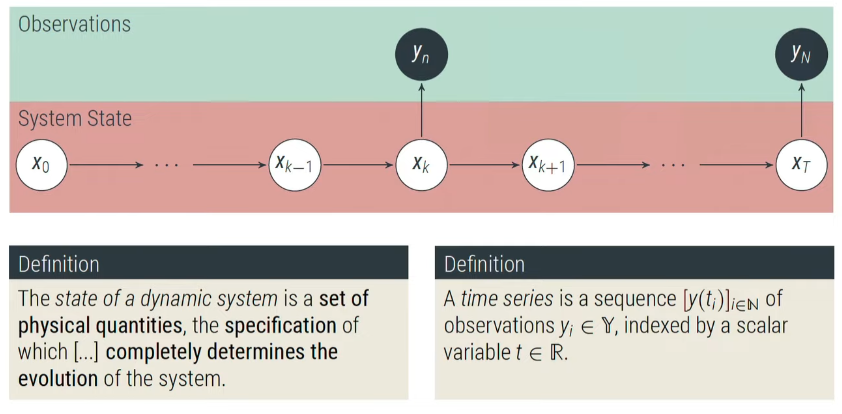
\includegraphics[scale=0.6]{./images/state_space/state_time_series.png}
% \end{figure}
% A probabilistic state-space model is a Bayesian model that defines
% \begin{itemize}
% 	\item An initial distribution $\rvx_0\sim p(\rvx_0)$ as a prior over the very first state, and for the state $\rvx_k\in \mathbb{R}^D$ and measurement $\rvy_k\in\mathbb{R}^d$ at time step $k$.
% 	\item A dynamics model as the prior over the (forward) state transitions.
% 		$$\rvx_k\sim p(\rvx_k|\rvx_{k-1}), $$
% 	\item A measurement model is a generative model for observations of the latent state.
% 		$$\rvy_k\sim p(\rvy_k|\rvx_{k}), $$

For a continuous-time system, the state-space model is typically expressed as follows:
% \end{itemize}
\begin{align*}
	\dot{x}(t) &= {A}x(t)+{B}u(t),\\
	% \frac{dX}{dt} &= {A}X+{B}U,\\
	y(t) &= {C}x(t)+Du(t).
\end{align*}
The first and the second equations are known as \textit{state equation} and \textit{output equation}, respectively. The state equation tells us that how the state vector changes with the state vector and the (external) input. 

\begin{itemize}
	\item $x(t)\in \mathbb{R}^n$: A state vector. This variable describes the state of the system at any given time.
	\item $\dot{x}\in \mathbb{R}^n$: state derivative \ie $\big(\frac{dX}{dt}\big)$ represents the changes of the state vector. You can notice that this is a linear combination of state vector and the input vector. 
	\item $u\in \mathbb{R}^m$: An external input affecting the system.
	\item $y\in \mathbb{R}^p$: An (Observed) Output.
	\item $A\in \mathbb{R}^{n\times n}$: A state matrix. This matrix describes how the state vector influences the changes of the state vector. 
	\item $B\in \mathbb{R}^{n\times m}$: An input matrix. This matrix describes how the (external) input vector influences the changes of the state vector. 
	\item $C\in \mathbb{R}^{p\times n}$: An output matrix. Typically, an identity matrix ($I$).
	\item $D\in \mathbb{R}^{p\times m}$: A feedthrough (or direct transmission) matrix. Typically, zeros
\end{itemize}

\subsection{Example: Mass-Spring-Damper System} 

Let's consider a simple example of a mass-spring-damper system, which can be described by the second-order differential equation.

The mass-spring-damper system is a common mechanical system that consists of three main components:
\begin{itemize}
	\item  Mass (\(m\)): A mass that can move along a straight line.
	\item  Spring (\(k\)): A spring that exerts a force proportional to its displacement from its equilibrium position (Hooke's Law).
	\item  Damper (\(c\)): A damping element (like a shock absorber) that exerts a force proportional to the velocity of the mass (damping force).
\end{itemize}

\begin{figure}[h]
	\centering
	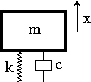
\includegraphics[scale=2.0]{./images/state_space/mass_spring.pdf}
\end{figure}

\paragraph{System Dynamics} The dynamics of this system can be described by Newton's second law of motion, which states that the sum of forces acting on the mass is equal to the mass times its acceleration (\(F = ma\)).

\paragraph{Differential Equation} For a mass-spring-damper system, the forces are:
\begin{itemize}
	\item Spring Force: \( F_{\text{spring}} = -kx(t) \), where \( x(t) \) is the displacement of the mass from its equilibrium position. The proportional constant $k$ is called the spring constant. It is a measure of the spring's stiffness.
	\item Damping Force: Damping forces are a special type of force that are used to slow down or stop a motion.  \( F_{\text{damper}} = -c\dot{x}(t) \), where \( \dot{x}(t) \) is the velocity of the mass (or object). Note that $\dot{x}(t)=dx(t)/dt$.
	\item External Force: \( F(t) \), an external force applied to the mass.
\end{itemize}

By summing these forces, we get:
\[ m\ddot{x}(t) = -kx(t) - c\dot{x}(t) + F(t). \]
To explain, the external force is stretching the spring, and the damper and the spring force are pulling the mass. Rearranging this, we get the second-order differential equation:
\[ m\ddot{x}(t) + c\dot{x}(t) + kx(t) = F(t) \]

\paragraph{State-Space Representation} To convert this second-order differential equation into a state-space representation, we need to express it as a system of first-order differential equations.

\paragraph{Defining State Variables} We introduce two state variables:
\begin{itemize}
	\item \( x_1(t) = x(t) \): the position of the mass.
	\item \( x_2(t) = \dot{x}(t) \): the velocity of the mass.
\end{itemize}

Now, we can write the original second-order equation as two first-order equations:
\[ \dot{x}_1(t) = x_2(t) \]
\[ \dot{x}_2(t) = \frac{1}{m}F(t) - \frac{k}{m}x_1(t) - \frac{c}{m}x_2(t) \]

\paragraph{Matrix Form} We can express these equations in matrix form:

\[ \begin{bmatrix} \dot{x}_1(t) \\ \dot{x}_2(t) \end{bmatrix} = \begin{bmatrix} 0 & 1 \\ -\frac{k}{m} & -\frac{c}{m} \end{bmatrix} \begin{bmatrix} x_1(t) \\ x_2(t) \end{bmatrix} + \begin{bmatrix} 0 \\ \frac{1}{m} \end{bmatrix} F(t) \]

This is the state-space form:
\[ \dot{x}(t) = Ax(t) + Bu(t) \]

Where:
\begin{itemize}
	\item \( x(t) = \begin{bmatrix} x_1(t) \\ x_2(t) \end{bmatrix} \) is the state vector.
	\item \( u(t) = F(t) \) is the input (external force).
	\item \( A = \begin{bmatrix} 0 & 1 \\ -\frac{k}{m} & -\frac{c}{m} \end{bmatrix} \) is the state matrix.
	\item \( B = \begin{bmatrix} 0 \\ \frac{1}{m} \end{bmatrix} \) is the input matrix.
\end{itemize}

\paragraph{Output Equation} 

If we consider the output to be the position of the mass (\( x_1(t) \)), the output equation is:

\[ y(t) = \begin{bmatrix} 1 & 0 \end{bmatrix} \begin{bmatrix} x_1(t) \\ x_2(t) \end{bmatrix} \]

So, the output equation is:

\[ y(t) = Cx(t), \]
Where \( C = \begin{bmatrix} 1 & 0 \end{bmatrix} \).

\paragraph{Full State-Space Model}

Combining the state and output equations, we get the full state-space representation:

\[ \dot{x}(t) = \begin{bmatrix} 0 & 1 \\ -\frac{k}{m} & -\frac{c}{m} \end{bmatrix} x(t) + \begin{bmatrix} 0 \\ \frac{1}{m} \end{bmatrix} u(t) \]
\[ y(t) = \begin{bmatrix} 1 & 0 \end{bmatrix} x(t) \]

In sum,
\begin{itemize}
	\item State variables: \( x_1(t) = x(t) \) (position), \( x_2(t) = \dot{x}(t) \) (velocity)
	\item Input: \( u(t) = F(t) \) (external force)
	\item Output: \( y(t) = x(t) \) (position)
	\item State equation: \( \dot{x}(t) = Ax(t) + Bu(t) \)
	\item Output equation: \( y(t) = Cx(t) \)
\end{itemize}

This state-space model describes how the position and velocity of the mass change over time in response to an external force.

% \[ m\ddot{x}(t) + c\dot{x}(t) + kx(t) = F(t) \]
% Where:
% \begin{itemize}
% 	\item \( m \) is the mass.
% 	\item \( c \) is the damping coefficient.
% 	\item \( k \) is the spring constant.
% 	\item \( x(t) \) is the displacement.
% 	\item \( F(t) \) is the external force applied.
% \end{itemize}


\subsection{Stability}

The linear state space model is stable if all eigenvalues of $A$ are negative real numbers or have negative real parts to complex number eigenvalues. If all real parts of the eigenvalues are negative then the system is stable, meaning that any initial condition converges exponentially to a stable attracting point. If any real parts are zero then the system will not converge to a point and if the eigenvalues are positive the system is unstable and will exponentially diverge.

% \subsection{First Order System in State Space}

% Let's consider an example to transform a first order linear system (without time delay):
% \begin{align*}
% 	\tau_{p}\frac{dy}{dt} &= -y+K_pu,\\
% \end{align*}
% where $\tau_{p}$ and $K_p$ are time constant and gain, respectively. Then, we can transform it into a state space form as follows:
% \begin{align*}
% 	\dot{x}&= \bigg[-\frac{1}{\tau_p}\bigg]x+\bigg[\frac{K_p}{\tau_p}\bigg]u,\\
% 	y &= [1]x+[0]u\\
% 	  &= x.
% \end{align*}
% Here, $A=-\frac{1}{\tau_p}$, $B = \frac{K_p}{\tau_p}$, $C=1$, and $D=0$. We can solve such model by using various methods like Laplace transform. 


% If the eigenvalues of $A$ are all smaller than $0$, then the system is called \textit{stable}. 

% \begin{itemize}
% 	\item $X\in \mathbb{R}^n$ and ${dX}/{dt}$ are the state vector and the differential state vector, respectively. 
% 	\item $U$ and $Y$ are scalar input vector and scalar output vector, respectively. 
% 	\item $A$ is the system matrix.
% 	\item $B$ and $C$ are the input and the output matrices.
% 	\item $D$ is the feed-forward matrix.
% \end{itemize}

\section{Legendre Memory Units}
\label{sec:nlp_lmu}


\section{Efficiently Modeling Long Sequences with Structured State-Spaces}
\label{sec:nlp_ssm}
The Linear State-Space Layer (LSSL) is a simple sequence model that maps a one-dimensional function  or sequence $u(t)\to y(t)$ through an implicit state $x(t)$ by simulating a linear continuous-time state-space representation in discrete-time
\begin{align*}
	x'(t) &= \mathbf{A}x(t)+\mathbf{B}u(t),\\
	y(t) &= \mathbf{C}x(t)+\mathbf{D}u(t).
\end{align*}

The first equation maps a single dimensional input signal $u(t)$ (or sequence) to an $N$-dim latent state (or hidden state) $x'(t)$ with the current state $x(t)$. The $\mathbf{A}$ and $\mathbf{B}$ can be considered as an non-linear mapping or transition matrices (\ie learnable parameters) to reflect the impact of the current state and the input, respectively. Finally, we project the input and the updated state to a one-dim output signal $y(t)$ (\ie sequence).  

Our goal is to simply use the SSM as a black-box representation in a deep sequence model, where $\rmA, \rmB, \rmC$, and $\rmD$ are parameters learned by gradient descent. We will omit the parameter $\rmD$ for exposition (or equivalently, assume $\rmD=0$, because the term $\rmD u$ can be viewed as a \textit{skip connection} and is easy to compute).

An SSM maps a input $u(t)$ to a state representation vector $x(t)$ and an output $y(t)$. For simplicity, we assume the input and output are one-dimensional, and the state representation is $N$-dimensional. The first equation defines the change in $x(t)$ over time.

\paragraph{Discretization} Then the discrete-time state-space model is given by
\begin{align*}
	x'(t) &= \overline{\mathbf{A}}x(t)+\overline{\mathbf{B}}u(t),\\
	y(t) &= \mathbf{C}x(t)+\underbrace{\mathbf{D}u(t)}_{=0},
\end{align*}
where $\overline{\mathbf{A}} = \mathbf{I}+\Delta \mathbf{A}$ and $\Delta \mathbf{B}$. To see how $\overline{\mathbf{A}}$ is derived:

\begin{align*}
	x'(t) &= \overline{\mathbf{A}}x(t)+\overline{\mathbf{B}}u(t)\\
		  &= \lim_{\Delta\to 0} \frac{x(t+\Delta)-x(t)}{\Delta}.
\end{align*}
Thus, 
\begin{align*}
	x(t+\Delta)-x(t) = \Delta x'(t).
\end{align*}
Equivalently, 
\begin{align*}
	x(t+\Delta) = \Delta x'(t)+x(t). 
\end{align*}
Plugging $x'(t)$ into the above equation, we get:
\begin{align*}
	x(t+\Delta) &= \Delta (\mathbf{A}x(t)+\mathbf{B}u(t)) +x(t) \\
				&= \underbrace{(\mathbf{I}+\Delta \mathbf{A})}_{\overline{\mathbf{A}}}x(t)+\underbrace{\Delta \mathbf{B}}_{\overline{\mathbf{B}}}u(t).
\end{align*}
We can say $x(t+\Delta)=x(t+1)$, since it is the next state we care. Thus, 
\begin{align*}
	x(t+1)= (\mathbf{I}+\Delta \mathbf{A})x(t)+\Delta \mathbf{B}u(t).
\end{align*}




\begin{figure}[h]
	\centering
	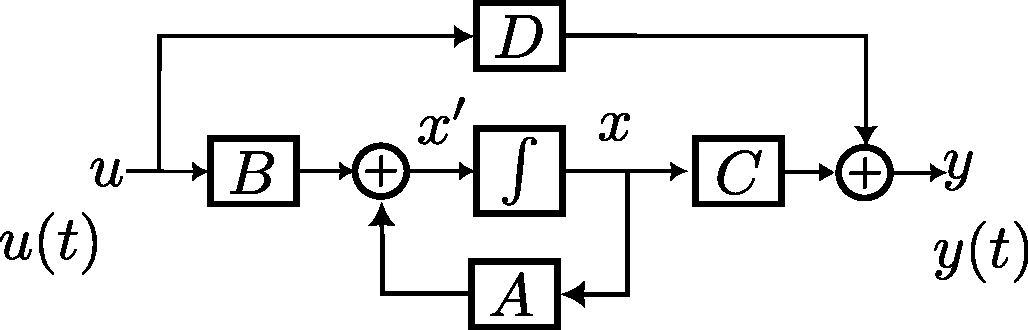
\includegraphics[scale=0.6]{./images/nlp/ssm.pdf}
	\caption{S4 Model}
	\label{fig:nlp_s4_model}
\end{figure}

We can represent the update process as follows:

At $t=0$
\begin{align*}
	x(0) &= \overline{\mathbf{B}}u(0),\\
	y(0) &= \mathbf{C}x(0)
\end{align*}

At $t=1$
\begin{align*}
	x(1) &= \overline{\mathbf{A}}x(0)+\overline{\mathbf{B}}u(1),\\
	y(1) &= \mathbf{C}x(1)
\end{align*}

At $t=2$
\begin{align*}
	x(2) &= \overline{\mathbf{A}}x(1)+\overline{\mathbf{B}}u(2),\\
	y(2) &= \mathbf{C}x(2).
\end{align*}
Note that this update process is equivalent to the RNN's update process. 

\paragraph{As a Convolution} 
The above process can be viewed as an one-dimensional convolution. 

\begin{align*}
	x(0) &= \overline{\mathbf{B}}u(0),\\
	y(0) &= \mathbf{C}x(0) = \mathbf{C}\overline{\mathbf{B}}u(0)\\
		 &\\
	x(1) &= \overline{\mathbf{A}}x(0)+\overline{\mathbf{B}}u(1)=\overline{\mathbf{A}}\overline{\mathbf{B}}u(0)+\overline{\mathbf{B}}u(1)\\
	y(1) &= \mathbf{C}x(1) = \mathbf{C}(\overline{\mathbf{A}}\overline{\mathbf{B}}u(0)+\overline{\mathbf{B}}u(1)) = \mathbf{C}\overline{\mathbf{A}}\overline{\mathbf{B}}u(0)+\mathbf{C}\overline{\mathbf{B}}u(1)\\
		 &\\
	x(2) &= \overline{\mathbf{A}}x(1)+\overline{\mathbf{B}}u(2)=\overline{\mathbf{A}}(\overline{\mathbf{A}}\overline{\mathbf{B}}u(0)+\overline{\mathbf{B}}u(1))+\overline{\mathbf{B}}u(2)=\overline{\mathbf{A}}^2\overline{\mathbf{B}}u(0)+\overline{\mathbf{A}}\overline{\mathbf{B}}u(1)+\overline{\mathbf{B}}u(2)\\
	y(2) &= \mathbf{C}x(2)=\mathbf{C}(\overline{\mathbf{A}}^2\overline{\mathbf{B}}u(0)+\overline{\mathbf{A}}\overline{\mathbf{B}}u(1)+\overline{\mathbf{B}}u(2))=\mathbf{C}\overline{\mathbf{A}}^2\overline{\mathbf{B}}u(0)+\mathbf{C}\overline{\mathbf{A}}\overline{\mathbf{B}}u(1)+\mathbf{C}\overline{\mathbf{B}}u(2)\\
\end{align*}
We get a general formula:
\begin{align*}
	y(t) &= \mathbf{C}\overline{\mathbf{A}}^t\overline{\mathbf{B}}u(0)+\mathbf{C}\overline{\mathbf{A}}^{t-1}\overline{\mathbf{B}}u(1)+\dots+\mathbf{C}\overline{\mathbf{B}}u(t)\\
		 &= \sum_{t=0}^T \mathbf{C}\overline{\mathbf{A}}^{T-t}\overline{\mathbf{B}}u(t)
\end{align*}
It turns out that the above equation is a one-dimensional convolution by a Kernel $K$:
\begin{align*}
	y = x*\overline{K}.
\end{align*}
Let's say the kernel size is 4 with zero-padding,  (See \Cref{fig:mamba_conv}).

\begin{figure}[h]
	\centering
	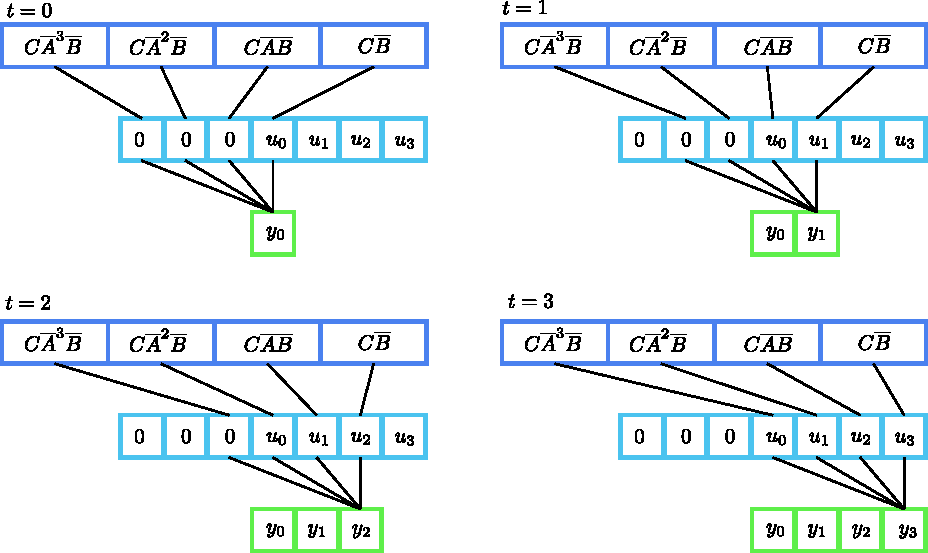
\includegraphics[scale=0.95]{./images/state_space/mamba_conv.pdf}
	\caption{}
	\label{fig:mamba_conv}
\end{figure}

During training, we can train the model as a convolutional neural network so that we can leverage the parallel training. During inference (\ie decoding stage), we can switch to the recurrent mode for near-constant time inference. Please note here, that if you look at the kernels you can see that they are fixed. And since the kernels are fixed, so we can also term these models as \textit{time-invariant} SSMs. 


https://blog.premai.io/s4-and-mamba/





